\documentclass{beamer}					% Document class

\usepackage[english]{babel}				% Set language
\usepackage[utf8x]{inputenc}			% Set encoding

% 加入 listings 套件
\usepackage{listings}
\usepackage{xcolor}

% 設定 listings 樣式
\lstset{
    language=R,
    basicstyle=\ttfamily\small,
    backgroundcolor=\color{gray!10},
    frame=single,
    breaklines=true,
    showstringspaces=false,
    keywordstyle=\color{blue},
    commentstyle=\color{green!50!black},
    stringstyle=\color{red},
    numbers=none,
    xleftmargin=10pt,
    xrightmargin=10pt,
    framexleftmargin=5pt,
    framexrightmargin=5pt
}

\mode<presentation>						% Set options
{
  \usetheme{default}					% Set theme
  \usecolortheme{default} 				% Set colors
  \usefonttheme{default}  				% Set font theme
  \setbeamertemplate{caption}[numbered]	% Set caption to be numbered
}

\usepackage{graphicx}					% For including figures
\graphicspath{{figure/}}				% Shared figure folder for all labs
\usepackage{booktabs}					% For table rules
\usepackage{hyperref}					% For cross-referencing
\usepackage{subcaption}  % 記得加在 preamble
\usepackage{multicol}

\title{Descriptive Statistics}	% Presentation title
\author{Rex Shao-Yu Wang}								% Presentation author
\institute{Department of Agronomy, National Taiwan University}					% Author affiliation
\date{March 16, 2026}									% Today's date	

\begin{document}

% Title page
\begin{frame}
  \titlepage
\end{frame}

% Outline
\begin{frame}{Outline}
  \tableofcontents
\end{frame}

\section{Import Data}
\begin{frame}[fragile]{Import Data}
Usually, you won't type in data manually; you'll get it from a file
\begin{lstlisting}
# Load a package
install.package("tidyverse")
library(tidyverse)

# Read a csv file
read_csv("file.csv")

#Read a txt file
read_delim("file.txt")

# Read an excel file
read_excel("file.xlsx") 

\end{lstlisting}

Example: iris data set
\begin{lstlisting}
iris_data <- read_csv("file_path")
\end{lstlisting}
\end{frame}

\begin{frame}{How to Find the File's Path}
    \begin{description}
        \item[\textbf{Mac OS}] \hfill \\
        Find your file $\rightarrow$ \textbf{Right-click} $\rightarrow$ Press \texttt{Option} key $\rightarrow$ Select \textbf{“Copy as Pathname”}
        
        \vspace{1.5em} % 增加間距避免太擠
        
        \item[\textbf{Windows}] \hfill \\
        Find your file $\rightarrow$ \textbf{Right-click} $\rightarrow$ Select \textbf{“Copy as path”} \\
        \quad {\small (Note: You may need to click “Show more options” first on Win11)}
    \end{description}

    \vspace{2em}
    
    \begin{exampleblock}{Pro Tip}
        In R, remember to change backslashes \texttt{\textbackslash} to forward slashes \texttt{/} or use double backslashes \texttt{\textbackslash\textbackslash} for Windows paths!
    \end{exampleblock}
\end{frame}

\begin{frame}{Other way to import data (User Friendly)}
File $\to$ Import Dataset $\to$ From Text (readr)
\begin{figure}
    \centering
    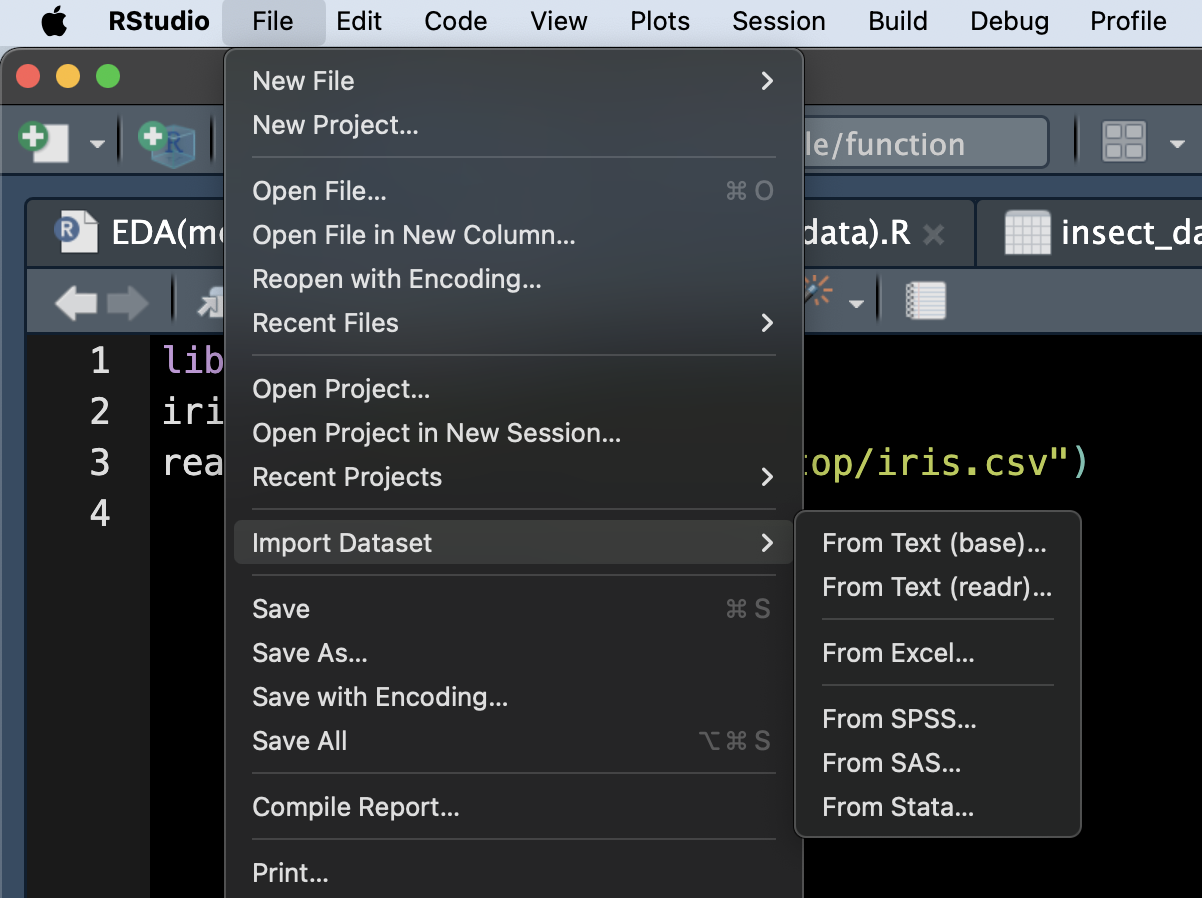
\includegraphics[width=0.8\linewidth]{Screenshot 2026-03-14 at 10.05.51 PM.png}
\end{figure}
\end{frame}

\begin{frame}{Other way to import data}
Click Browser to choose your data $\to$ Click Import to put your data into R environment
\begin{figure}
    \centering
    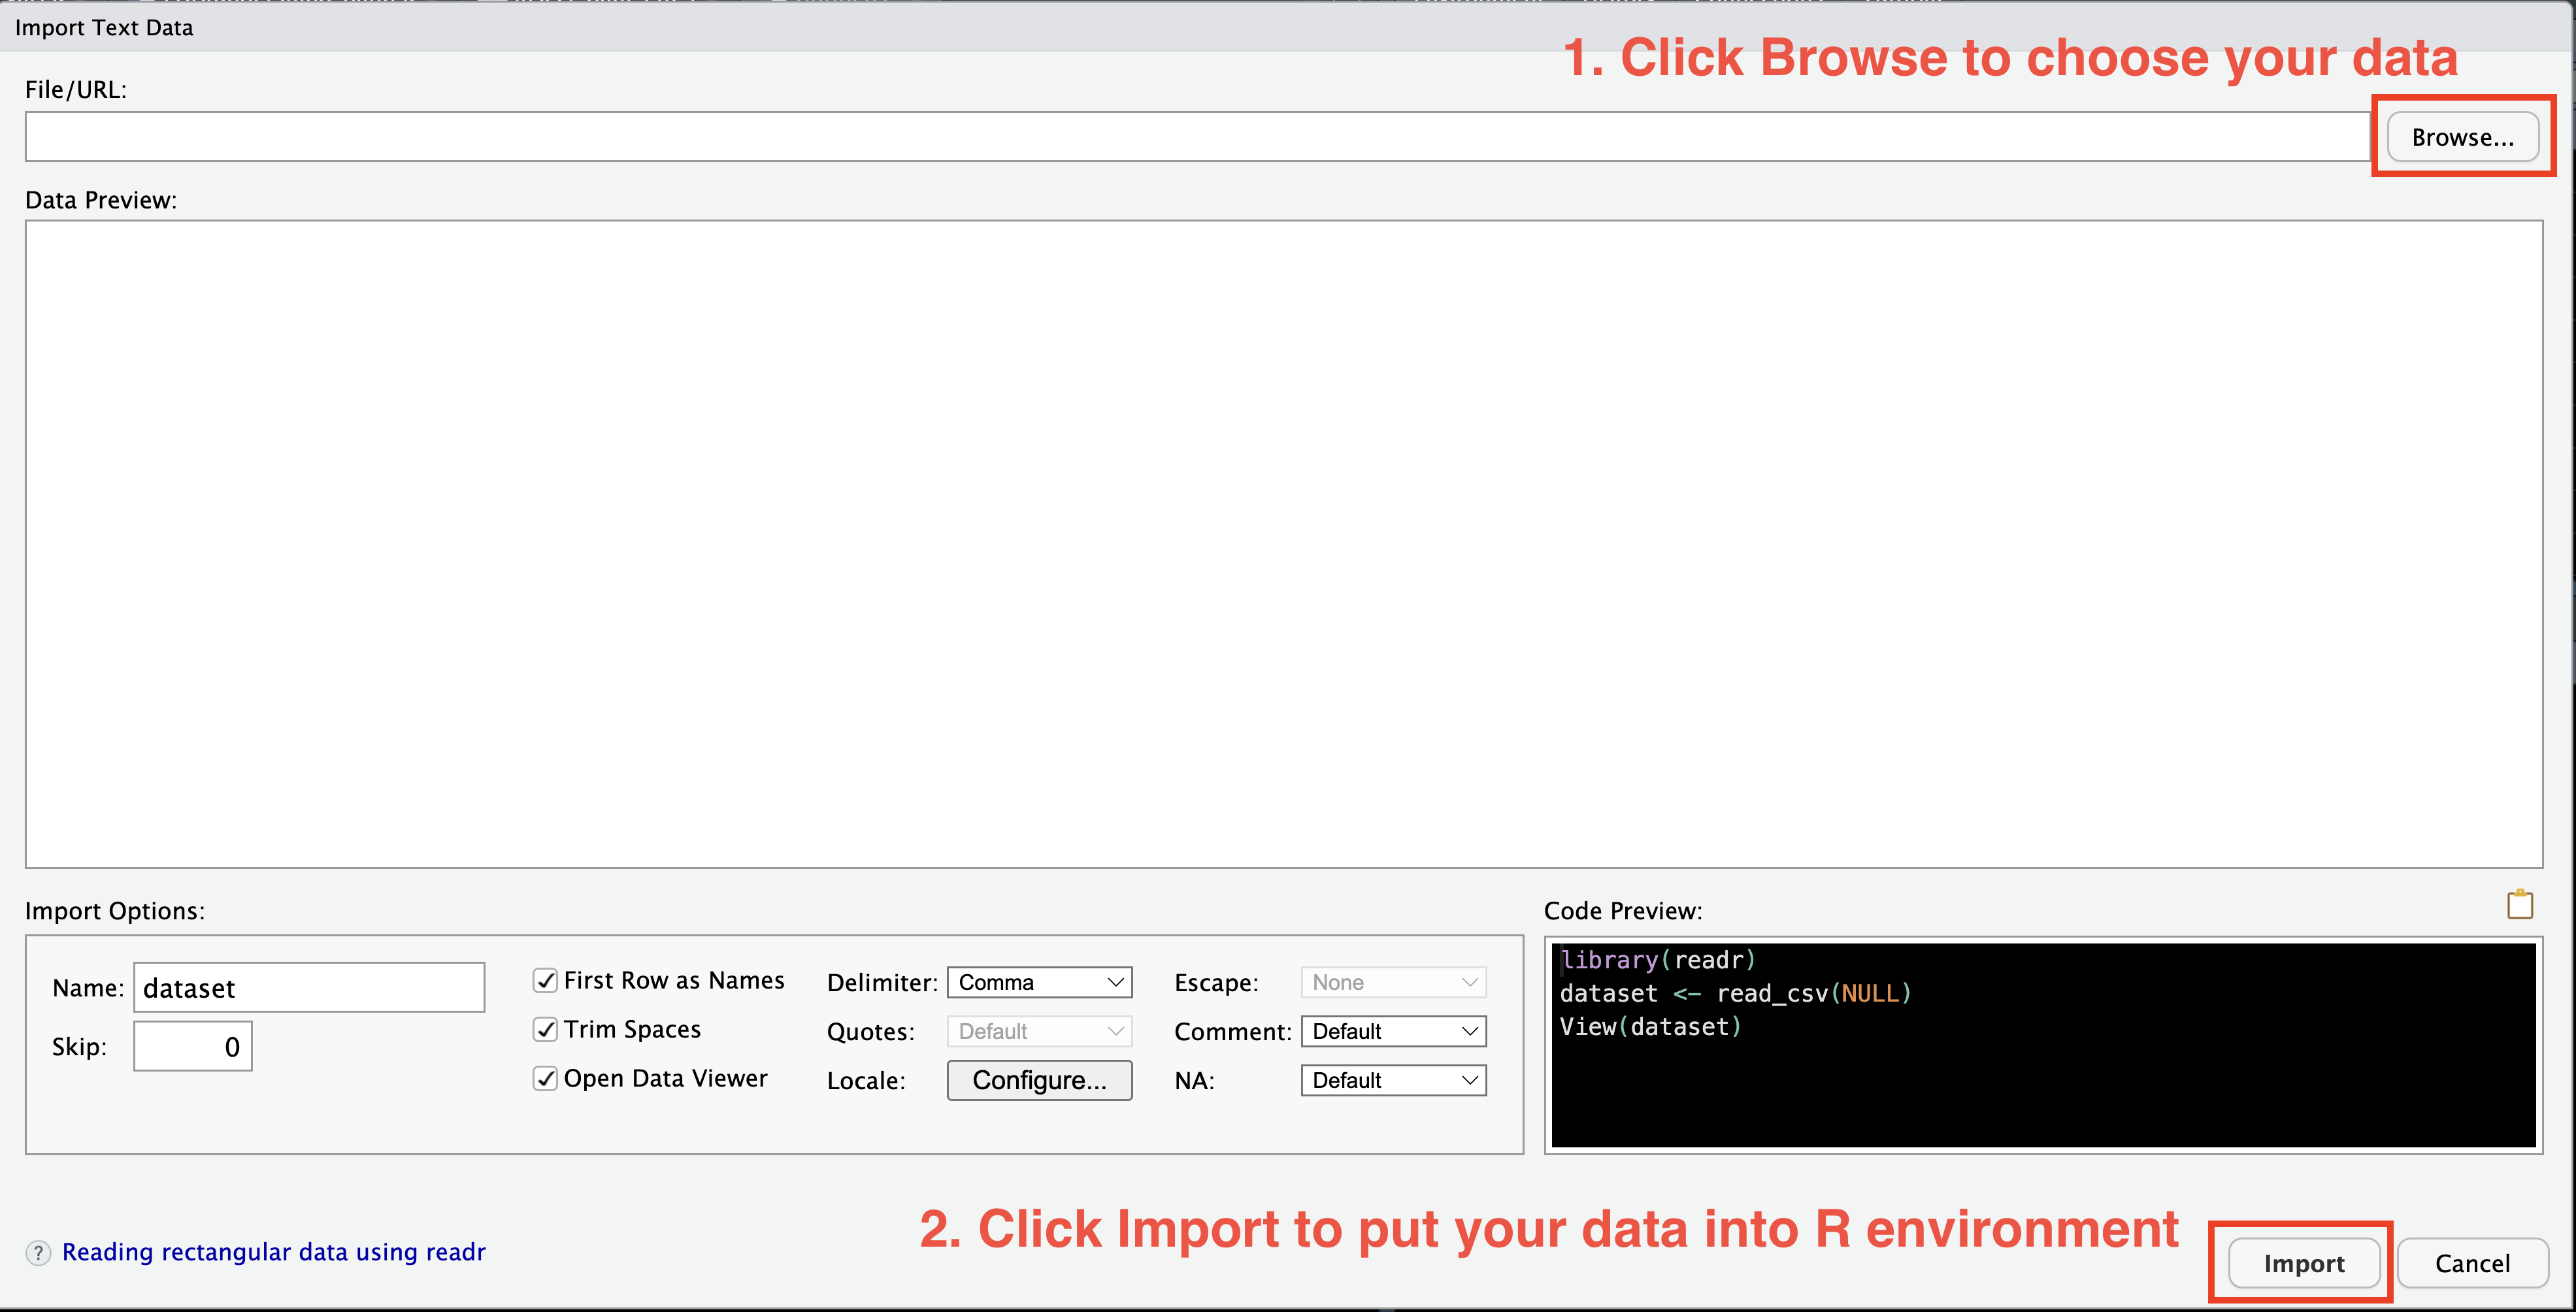
\includegraphics[width=1\linewidth]{Screenshot 2026-03-15 at 12.25.07 AM.png}
\end{figure}
\end{frame}

\begin{frame}[fragile]{Check the iris dataset}
\texttt{head()}: show the first six rows of data\\
\texttt{tail()}: show the last six rows of data\\
\texttt{str()}: structure of data
\vspace{10pt}
\begin{lstlisting}
head(iris_data)
head(iris_data, n = 10)

tail(iris_data)
tail(iris_data, n = 25)

str(iris_data)
\end{lstlisting}
\end{frame}

\section{Descriptive Statistics}
\begin{frame}{Descriptive Statistics}
    \begin{columns}[c] % [c] 使左右內容垂直居中對齊

        \column{0.5\textwidth}
        \begin{itemize}
            \item \texttt{min()}: Minimum
            \item \texttt{max()}: Maximum
            \item \texttt{median()}: Median
            \item \texttt{quantile(,p=)}: Quantile
            \item \texttt{mean()}: Average
            \item \texttt{sum()}: Total
            \item \texttt{var()}: Variance
            \item \texttt{sd()}: Standard Deviation
            \item \texttt{summary()}: Overview
        \end{itemize}
        
        \column{0.5\textwidth}
        \begin{figure}
            \centering
            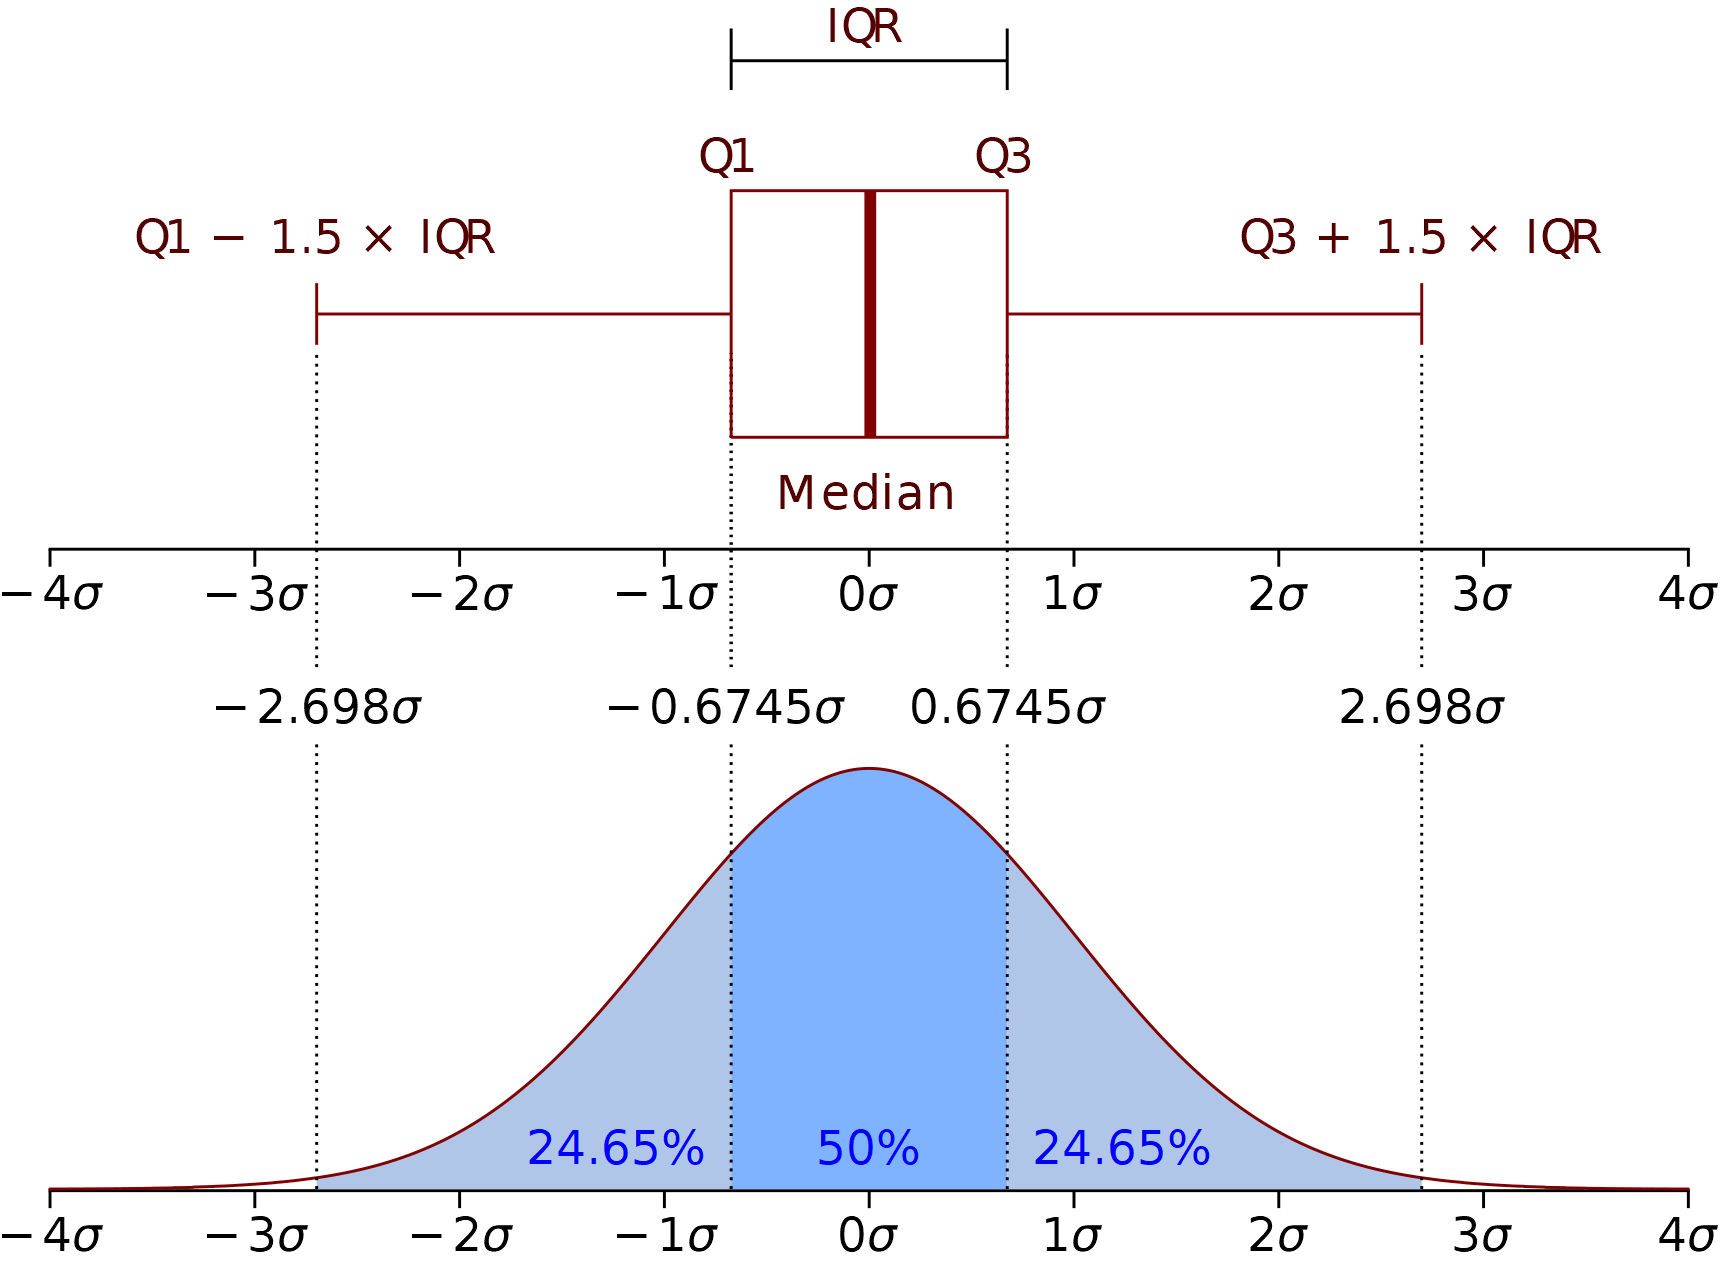
\includegraphics[width=\linewidth]{interquartile-range-20190130-01.png}
        \end{figure}
        
    \end{columns}
\end{frame}

\begin{frame}[fragile]{Box Plot}
    \textbf{Function:} \texttt{boxplot(data)} \\
    \textbf{Example:}
    \begin{lstlisting}[language=R, basicstyle=\small\ttfamily]
boxplot(iris_data$Petal.Length, 
        main = "Boxplot of Petal Length",
        xlab = "Petal Length (cm)", 
        ylab = "", 
        horizontal = TRUE) 
    \end{lstlisting}
    \begin{figure}[c]
        \centering
        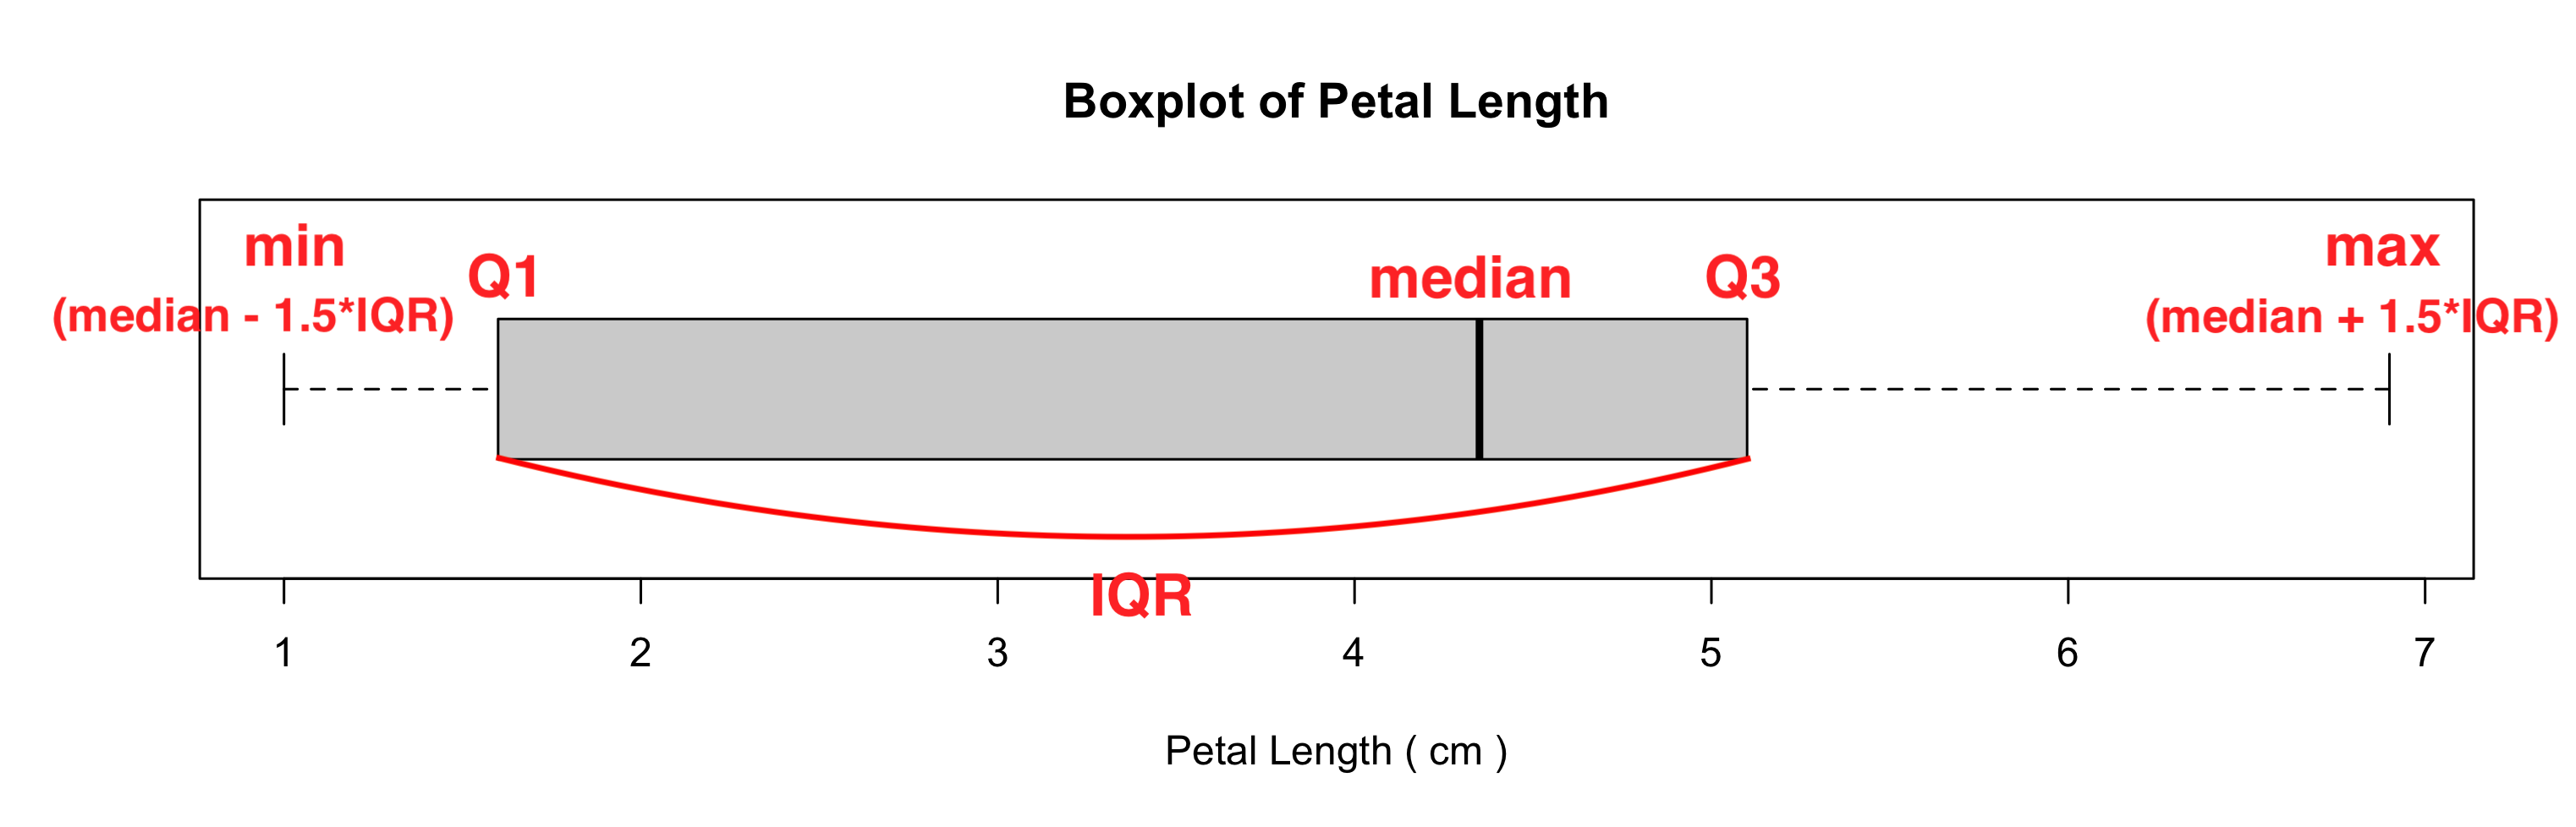
\includegraphics[width=1.05\linewidth]{Boxplot_horizontal.png}
    \end{figure}
\end{frame}

\begin{frame}{Getting help}
\begin{itemize}

    \item \texttt{help(mean)}: help about function mean()
    \item \texttt{?mean}: Same. Help about the function mean()
    \item \texttt{example(mean)}: Show an example of function mean()
    \item \texttt{help.search("mean")}: Get help on a specific topic 
    
\end{itemize}
    
\end{frame}

\section{Practice}
\begin{frame}{Practice}
\begin{itemize}

\item Read the data "students.csv" into R and name it as "student\_data" 
\item Compute \textbf{minimum}, \textbf{maximum}, \textbf{mean}, \textbf{variance}, and \textbf{standard deviation} of math score
\item Draw a \textbf{boxplot} of reading score
\end{itemize}

    
\end{frame}
\end{document}
